%% IEEE Transactions on Dependable and Secure Computing -- regular paper submission.
%% Build: pdflatex main && bibtex main && pdflatex main && pdflatex main
\documentclass[10pt,journal,compsoc]{IEEEtran}
% Shared preamble for the IEEE TDSC manuscript (main.tex) and its supplementary material (supplement.tex).
\usepackage[T1]{fontenc}
\usepackage{newtxtext,newtxmath}
\usepackage[numbers,sort&compress]{natbib}
% IEEE style sets the reference list in footnote size; natbib replaces IEEEtran's
% thebibliography environment, so restore the font and tight item spacing here.
\renewcommand{\bibfont}{\footnotesize\setlength{\emergencystretch}{3em}}
\setlength{\bibsep}{1.5pt plus 0.5pt}
\usepackage{amsmath}
\let\openbox\relax
\usepackage{amsthm}
\usepackage{graphicx}
\usepackage{booktabs}
\usepackage{array}
\usepackage{tabularx}
\usepackage{xcolor}
\usepackage{tikz}
\usepackage[hyphens]{url}
\usepackage[hidelinks,breaklinks=true]{hyperref}
\usepackage{microtype}
\graphicspath{{figures/}}

\theoremstyle{plain}
\newtheorem{theorem}{Theorem}
\newtheorem{proposition}{Proposition}
\newtheorem{lemma}{Lemma}
\newtheorem{corollary}{Corollary}
\theoremstyle{definition}
\newtheorem{definition}{Definition}
\newtheorem{assumption}{Assumption}
\newtheorem{example}{Example}
\theoremstyle{remark}
\newtheorem{remark}{Remark}

\newcommand{\A}{A}
\newcommand{\Astar}{A^{*}}
\newcommand{\Aomega}{A^{\omega}}
\newcommand{\D}{\mathcal{D}}
\newcommand{\Th}{\mathcal{T}}
\newcommand{\RA}{\mathsf{RA}}
\newcommand{\Good}{\mathrm{Good}}
\newcommand{\Bad}{\mathrm{Bad}}
\newcommand{\Pdist}{\mathbb{P}}
\newcommand{\E}{\mathbb{E}}
\newcommand{\allow}{\mathsf{allow}}
\newcommand{\block}{\mathsf{block}}
\newcommand{\subst}{\mathsf{sub}}
\newcommand{\Dec}{\mathrm{Dec}}
\newcommand{\noop}{\bot}
\newcommand{\erase}{\mathsf{ext}}
\newcommand{\ROC}{\mathrm{roc}}
\newcommand{\eff}{\mathrm{eff}}
\newcommand{\indep}{\perp\!\!\!\perp}
\DeclareMathOperator*{\argmin}{arg\,min}
\DeclareMathOperator*{\argmax}{arg\,max}
\newcommand{\PSPACE}{\textsc{pspace}}
\newcommand{\NP}{\textsc{np}}
% Run-in paragraph headings in bold (IEEEtran compsoc's default \paragraph is plain roman,
% indistinguishable from body text); same spacing and run-in period as the class default.
\setcounter{secnumdepth}{3}% journal mode would otherwise number run-in \paragraph headings
\makeatletter
\def\paragraph{\@startsection{paragraph}{4}{\parindent}{0ex plus 0.1ex minus 0.1ex}{0ex}{\normalfont\normalsize\bfseries}}
\makeatother
% Avoid stretched vertical gaps when a heading or float moves to the next column.
\raggedbottom
% Let TeX fix the rare line that would otherwise overflow (e.g., long reference titles).
\setlength{\emergencystretch}{1em}

% Public artifact (code, cached judge scores); complete proofs and extended experiments are in
% the separately submitted supplementary material (supplement.tex).
\newcommand{\artifactURL}{\url{https://github.com/shawnray-research/certified-agent-guardrails/tree/tdsc}}

\hypersetup{pdftitle={What Can Be Enforced? Limits of Runtime Guardrails for Tool-Using LLM Agents},
  pdfauthor={Shawn Ray},
  pdfkeywords={AI agent security, runtime enforcement, guardrails, prompt injection, security automata, conformal risk control, large language models}}
\begin{document}
\bstctlcite{IEEEexample:BSTcontrol}
\title{What Can Be Enforced? Limits of Runtime Guardrails for Tool-Using LLM Agents}
\author{Shawn~Ray%
\IEEEcompsocitemizethanks{\IEEEcompsocthanksitem S.~Ray is with Carnegie Mellon University,
Pittsburgh, PA 15213, USA.\protect\\
E-mail: shawnray@cmu.edu\protect\\
An earlier version of this work is available as arXiv:2607.22868.}}
\markboth{IEEE Transactions on Dependable and Secure Computing}%
{Ray: What Can Be Enforced? Limits of Runtime Guardrails for Tool-Using LLM Agents}

\IEEEtitleabstractindextext{%
\begin{abstract}
LLM agents rely on runtime guardrails, judge-driven gates before irreversible tool calls, against
prompt injection, yet evaluations report violation rates, not what gates enforce or certify. We
delimit three boundaries. Expressiveness: relative to oracle predicates, a non-retracting gate enforces
exactly the nonempty safety policies whose good prefixes its register automaton recognizes, below edit automata.
Statistics: Neyman--Pearson gives the exact miss/false-block frontier of the gate's information and
conformal risk control a finite-sample certificate; judge-input rewrites add a robustness margin, and
choosing the violation voids both; once blocks change later proposals, only exploratory logs identify the
closed-loop frontier. Decidability: whether a policy can fire is undecidable with two zero-testable
counters, PSPACE-complete for a keyed-counter fragment, and NP-complete for caps, quotas, and
revocation. On AgentDojo, deterministic gates calibrated on 17--18 instruction-string violations to a
10\% miss target block at least 64\% of compliant instructions; given the user request and tool outputs
of replayed traces, hosted judges separate injected from compliant calls in the same context (AUC
.87--1.00) and block at most 16\% of the latter, yet rewriting injected text evades them on up to
12\% of flagged calls. Certificates must state the oracle interface, operating point, calibration
population, adversarial margin, and feedback model.

\end{abstract}
\begin{IEEEkeywords}
AI agent security, runtime enforcement, guardrails, prompt injection, security automata,
conformal risk control, large language models.
\end{IEEEkeywords}}

\maketitle
\IEEEdisplaynontitleabstractindextext
\IEEEpeerreviewmaketitle

\IEEEraisesectionheading{\section{Introduction}\label{intro:sec}}
\IEEEPARstart{L}{anguage-model} agents act through tools with irreversible effects (email,
payments, file edits) while reading untrusted content, so an attacker who
controls that content can steer the next tool call
\citep{greshake2023injection}. A common defense is a runtime guardrail: a
judge, often itself a language model, scores each proposed call, and a gate
blocks, rewrites, or escalates it before it executes
\citep{inan2023llamaguard,chennabasappa2025llamafirewall,agentspec2026,probguard2025,veriguard2025,agentc2025,wu2026provably}.
This gate is the security boundary between an injectable agent and
irreversible effects (Figure~\ref{fig:overview}). In the dependability
taxonomy of \citet{avizienis2004basic}, the gate is an error-detection and containment
mechanism in front of irreversible service: each miss lets a security or safety failure
through, and each false block is an omission failure that costs availability. Whether the
gate can justifiably be trusted therefore depends both on its error rates and on the fault
assumptions under which they are claimed.


Benchmark violation and false-positive rates do not say which policies a
gate can enforce at all, what a calibrated ``certificate'' guarantees, or
when that guarantee stops holding. For programs, the first question has a
classical answer: execution
monitors enforce only safety properties \citep{schneider2000enforceable}, and edit
automata enforce more by suppressing and reinserting actions
\citep{ligatti2005edit}. Agent gates depart from that setting in four ways: a fallible judge
decides the policy predicate (``does this body contain PII?''); effects are
irreversible, so the gate cannot buffer and retract as an edit automaton does, which
returns it to the execution-monitor (safety) regime of \citet{schneider2000enforceable};
actions carry unbounded data, which security automata already admit over countable
alphabets but which a deployed gate must represent finitely; and the attacker controls
part of what the judge sees. The safety half of our first result is therefore classical;
its contribution is the effect-trace, oracle-relative, register-automaton form:
characterizing the class a monitor with restricted state enforces is classical over finite
alphabets \citep{fong2004shallow,talhi2008memory}, and we carry it to keyed-counter register
automata over infinite data alphabets, relative to oracle bits. Each result states where it applies. ``Certified'' means
streamwise enforcement relative to fixed oracle predicates, or a marginal risk
bound under explicit stochastic assumptions, never universal semantic safety.

\begin{example}[Running example: an email/payments assistant]\label{ex:running}
An assistant acts for a user through tools such as
$\mathsf{send\_email}(\mathit{to},\mathit{body})$ and
$\mathsf{transfer}(\mathit{to},\mathit{amount})$, under three policies:
(P1)~never email a body containing PII to a recipient not on the approved list;
(P2)~never let cumulative transfer to any recipient exceed cap $c$ in a day bucket set by a trusted clock;
(P3)~after the user revokes access, send nothing further. P2 and P3 are
oracle-checkable data-carrying properties; P1 rests on the semantic predicate
``contains PII,'' which only a fallible judge evaluates.
\end{example}

\begin{figure}[t]
\centering
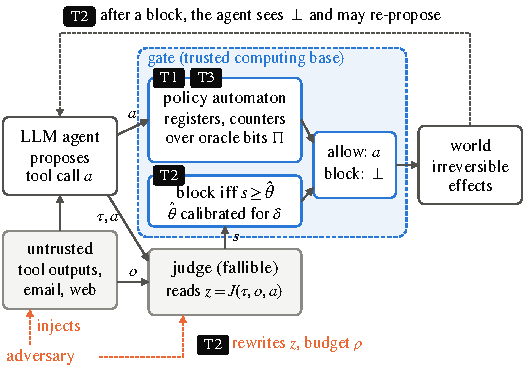
\includegraphics[width=\columnwidth]{overview}
\caption{A guarded tool-using agent. The agent, partly steered by untrusted input, proposes a
data-carrying tool call $a$. The gate (the trusted computing base) combines a policy automaton over
oracle bits $\Pi$ with a threshold test on a fallible judge's score $s$ of the judge-visible input $z$,
and either commits $a$ irreversibly or blocks it by committing the no-op $\bot$. T1: what the automaton
can enforce. T2: what a judge-based test can certify (frontier, calibration of $\hat\theta$, budget-$\rho$
rewrites of $z$, feedback). T3: whether a rule can ever fire, decided before deployment.}
\label{fig:overview}
\end{figure}

\paragraph{Three boundaries}
\emph{T1, expressiveness (\S\ref{sec:t1}).} Relative to fixed oracle predicates, a deterministic gate
enforces exactly the nonempty safety policies whose good prefixes its register automaton recognizes
(Theorem~\ref{thm:t1}), strictly fewer than edit automata (Proposition~\ref{prop:strict}): a gate that
cannot retract must refute violations on finite prefixes. P2 and P3 are inside this class; P1 needs a judge.
\emph{T2, statistics, adversaries, and feedback (\S\ref{sec:t2}).} With a judge, Neyman--Pearson gives the
exact miss/false-block frontier of the gate's information (Proposition~\ref{thm:frontier}) and conformal
risk control a finite-sample certificate (Theorem~\ref{thm:conformal}) that may be block-all; rewrites of
the judge's input within budget $\rho$ add a margin (Theorem~\ref{thm:adv}); once blocks change later
proposals, static scores and ungated logs cannot identify the closed-loop frontier
(Proposition~\ref{prop:feedback}), whereas exploratory blocking logs can, at a variance that may grow
exponentially in the horizon (Proposition~\ref{prop:explore}).
\emph{T3, decidability (\S\ref{sec:t3}).} Whether a rule can ever fire is undecidable with two
zero-testable counters (Proposition~\ref{thm:undec}), \PSPACE-complete for a keyed-counter fragment with data
registers, and \NP-complete for caps, quotas, and revocation without them, so one SMT query lints them (Theorem~\ref{thm:frag}). Table~\ref{tab:summary} gives each result's regime and what is
imported versus new.

% Summary of the three boundaries (journal version): what each result says, when it holds,
% what is imported versus new, and what it means for a deployment.
\begin{table*}[t]
\caption{The three boundaries at a glance. Each result holds only in its stated regime; the
evidence column points to the experiment that probes it.}
\label{tab:summary}
\centering\footnotesize
\setlength{\tabcolsep}{4pt}
\renewcommand{\arraystretch}{1.12}
\begin{tabularx}{\textwidth}{@{}>{\raggedright\arraybackslash}p{0.255\textwidth}>{\raggedright\arraybackslash}p{0.15\textwidth}>{\raggedright\arraybackslash}X>{\raggedright\arraybackslash}X>{\raggedright\arraybackslash}p{0.062\textwidth}@{}}
\toprule
Boundary and result & Regime & Imported ingredient $\rightarrow$ what is new & Consequence for deployments & Evidence\\
\midrule
\textbf{T1 expressiveness} (Thm.~\ref{thm:t1}, Prop.~\ref{prop:strict}): a deterministic gate
enforces exactly the nonempty safety policies with $\Good(P)\in\RA[\Th;\Pi]$, strictly fewer than
edit automata
& fixed oracle bits $\Pi$; irreversible commits; every proposal stream
& security, truncation, and bounded-memory automata
\citep{schneider2000enforceable,ligatti2005edit,talhi2008memory} $\rightarrow$
effect-trace, oracle-relative, keyed-counter register form over data-carrying actions
& compile caps, quotas, and revocation to exact gates; deferred commits belong in the tool
interface, not in the gate
& \S\ref{sec:q5}\\
\addlinespace
\textbf{T2 exogenous frontier} (Prop.~\ref{thm:frontier}, Cor.~\ref{cor:reduction}): the ROC of the
gate's information is the exact miss/false-block frontier
& one-step law independent of the gate
& Neyman--Pearson, Blackwell $\rightarrow$ the object guardrail benchmarks should report, lifted
to episodes
& no ensemble or wrapper on the same information beats it; report an operating point, not AUC
& \S\ref{exp:q1}\\
\addlinespace
\textbf{T2 certificate} (Thm.~\ref{thm:conformal}): calibrated per-step miss risk $\delta/H$ bounds
the unsafe-episode rate by $\delta$
& label-conditional exchangeability (Asm.~\ref{ass:benign})
& conformal risk control $\rightarrow$ per-step gate calibration on violating examples
& the bound is marginal and may be met only by blocking everything
& \S\ref{exp:q1}\\
\addlinespace
\textbf{T2 adversary} (Thm.~\ref{thm:adv}, Prop.~\ref{prop:zero-miss}, Cor.~\ref{cor:robust}):
the bound degrades to $\min\{1,\delta+H\bar\eta(\rho)\}$
& benign calibration; budget-$\rho$ judge-input rewrites (choosing the violation voids it)
& robust conformal prediction \citep{gendler2022robustconformal} $\rightarrow$ risk-level
margin-aware recalibration for discrete rewrites, valid once $\bar\eta(\rho)<\delta/H$ is verified
& benign calibration is not a security boundary; attacks can refute, never certify, a margin
& \S\ref{exp:q3}\\
\addlinespace
\textbf{T2 feedback} (Prop.~\ref{prop:feedback}, Cor.~\ref{cor:no-estimator},
Prop.~\ref{prop:explore}, Thm.~\ref{thm:sequential}): ungated logs do not identify the
closed-loop frontier; exploratory blocking does
& blocks change later proposals
& CPOMDP occupancy, off-policy overlap $\rightarrow$ non-identifiability for gated agents; occupancy
program for finite models
& evaluate in the loop, logging known block and allow probabilities; sample cost can grow like
$\varepsilon^{-H}$
& \S\ref{exp:q2}, \S\ref{exp:q4}\\
\addlinespace
\textbf{T3 decidability} (Prop.~\ref{thm:undec}, Thm.~\ref{thm:frag}): whether a policy can ever
fire is undecidable with two zero-testable counters, \PSPACE-complete for $\Th_0$, \NP-complete for caps, quotas, revocation
& static analysis of the policy specification
& Minsky machines, register-automaton \PSPACE-hardness \citep{demri2009ltl} $\rightarrow$ $\Th_0$ via exact cap saturation and a
one-witness reduction; Parikh phases for cap checks
& keep policy languages inside $\Th_0$ (caps, quotas, revocation: one SMT query) to ship a complete ``can this rule fire'' linter
& \S\ref{sec:q5}\\
\bottomrule
\end{tabularx}
\end{table*}


\paragraph{Empirical findings}
On AgentDojo \citep{debenedetti2024agentdojo} (\S\ref{sec:exp}), with 33 judge runs (32 models):
\begin{itemize}[\setlength{\IEEElabelindent}{0pt}\IEEEsetlabelwidth{$\bullet$}]
  \item \emph{Instruction strings make gates expensive.} After familywise correction only Claude
  Opus~5.5 (AUC $.929$, refusals counted as blocks; not if scored $.5$) beats Gemma-2-9B (AUC $.813$) in all
  three runs. At miss target $\delta=.10$, with 17--18 calibration violations per fold, even the best
  deterministic split-conformal gate blocks 64\% of compliant instructions (95\% CI 20--83\%; 11\% without the 7 goals whose text is benign), because $\hat\theta$ is then the single lowest violating calibration score, and every
  $\delta=.05$ gate is block-all; exact-level randomized calibration halves the cost (33\%).
  \item \emph{What the gate sees decides the frontier.} Given the user request and the tool outputs, the
  seven hosted judges separate injected from compliant calls in the same context with AUC $.872$--$.999$
  ($.621$--$.835$ for the same calls serialized alone), and gates cross-fitted over goals miss $.038$--$.098$ while
  blocking at most 5.3\% of clean compliant calls ($43.7$--$92.6\%$ without context).
  \item \emph{Context buys discrimination, not verified robustness.} In context, best-of-20 rewrites of the injection
  stably evade the $\delta=.10$ gate on 12 of 101 flagged calls for Claude Haiku~5.5 net of a clean-prompt null
  control, and on at most 6 for each other judge. On instruction strings, one predeclared 16-word suffix raises the miss rate at
  $\theta=.5$ by $.200$--$.657$ for 10 of 21 judges (no Claude or GPT judge), and an optimizing attacker
  evades even the gates that block $32$--$87\%$ of compliant instructions on 27--35\% of flagged violations.
  Attacks refute margins; they never certify one.
  \item \emph{Closed loop and cost.} A 3B-judge gate that drops 78\% of a local 7B agent's calls cuts attack
  success from $.047$ to $.004$ (descriptive; no A/A or random-drop control), and a compiled P2+P3 gate
  decides in under a microsecond, about $10^6$ times faster than a hosted judge call (\S\ref{sec:q5}).
\end{itemize}
A guardrail certificate therefore means little without its oracle interface, operating point,
calibration population, adversarial margin, and feedback model (\S\ref{sec:disc}).

\paragraph{Contributions} Beyond the imported ingredients named in Table~\ref{tab:summary}:
\begin{itemize}[\setlength{\IEEElabelindent}{0pt}\IEEEsetlabelwidth{$\bullet$}]
  \item \emph{An exact enforceability boundary} (\S\ref{sec:model}--\S\ref{sec:t1}): the oracle/judge
  split, the class a non-retracting register gate enforces over data-carrying effects, and a separation
  showing why the oracle interface must be action-local.
  \item \emph{An attack and feedback accounting for calibrated gates} (\S\ref{sec:t2}): benign calibration
  degrades to $\delta+H\bar\eta(\rho)$, margin-aware recalibration restores $\delta$ only for a verified
  margin, and closed-loop frontiers are identified by exploratory blocking but not by static scores or
  ungated logs.
  \item \emph{A decidable policy fragment} (\S\ref{sec:t3}): nontriviality is \PSPACE-complete for the fragment (hard via registers
  alone) and \NP-complete for caps, quotas, and revocation without registers.
  \item \emph{An evaluation} (\S\ref{sec:exp}) that separates calibration cost (33 judge runs), what the
  gate sees (tool calls with and without context), representation attacks, and closed-loop effects.
  \item \emph{A guardrail certificate card} (\S\ref{sec:disc}, Table~\ref{tab:card}): five fields every
  evaluation must report, each required by one of our results, with a template in the artifact.
\end{itemize}
Code, the curated probe, and cached judge scores are public\footnote{\artifactURL} (except the
source-role and closed-loop-rerun caches; Supplement~C); complete
proofs and extended experiments are in the supplementary material (Supplements~A--E).

\section{System and Threat Model}\label{sec:threat}

\paragraph{System and trusted computing base}
An agent acts for a user by proposing tool calls one at a time. A pre-execution gate sees
the committed effect history, the proposed action $a$, and the scores of $m$ judges, and
returns $\allow$, $\block$, or $\subst(a')$ before the action commits
(Def.~\ref{def:gate}). Commits are irreversible; blocking commits the no-op $\noop$, which
has no external effect. The agent may observe a block and change its later proposals; T1 abstracts
this feedback away and T2 models it as a decision-dependent kernel
(Def.~\ref{def:controlled}). The TCB consists of the gate code, its policy automaton, the
oracle predicate bits $\Pi$ when available, and trusted metadata (in the running example, a
trusted clock adapter for P2's day bucket and provenance labels that grant authority only to
user input). The agent is outside the TCB, so T1 quantifies over every proposal stream; the
judge is a black-box test with false-alarm rate $\alpha$ and miss rate $\beta$
(Def.~\ref{def:judge}). In the terminology of \citet{avizienis2004basic}, injected content
and judge errors are faults, a violating proposal that reaches the gate is an error, a
violating committed effect is a failure, and a false block is an omission failure.

\paragraph{Adversary}
The adversary controls untrusted content the agent reads (tool outputs, documents, email)
and uses it for indirect prompt injection \citep{greshake2023injection}. It has three
capabilities. (i)~\emph{Injection:} it chooses the injected content, and hence which violating
proposals the agent makes. (ii)~\emph{Knowledge:} it knows the policy, the scoring function, and
the threshold. (iii)~\emph{Judge-input rewriting} (Def.~\ref{def:adversary}): at deployment,
adaptively across steps, it may replace the judge-visible representation $z=J(\tau,o,a)$, with
$\tau$ the committed effect history and $o$ the untrusted context the judge reads, by any $z'$
with $d(z,z')\le\rho$, e.g., by inserting at most $\rho$ tokens into a tool-output field,
leaving the action, its effect, and its label unchanged; since tool outputs are attacker-written,
$\rho$ is limited in practice only by the field length, so a margin must be stated for the budget a
deployment admits. Calibration examples are benign. Theorem~\ref{thm:adv} prices only~(iii): it
requires that the violating proposals produced under~(i) remain label-conditionally exchangeable
with the calibration violations (Assumption~\ref{ass:benign}), and an adversary that uses~(i) to
choose or shift the induced violation, e.g., toward goals whose text reads as benign
(\S\ref{exp:q1}), voids that assumption and with it Theorems~\ref{thm:conformal}
and~\ref{thm:adv}. Our experiments (\S\ref{exp:q3}) instantiate only black-box members
of~(iii), which lower-bound $\bar\eta(\rho)$: they can refute a margin but never certify one. A deployed gate should treat a refusal or any other non-answer as a
block (fail-closed); \S\ref{sec:exp} states how our caches score refusals. Out of scope are
compromise of the gate, the oracle, or the trusted adapters; training-time poisoning of the
judge or of the calibration set; side channels; and adversarially induced false blocks (a
denial-of-service lever our bounds do not price).

\paragraph{Goals and what ``certified'' means}
The gate is a reference monitor for tool calls \citep{anderson1972planning}: we assume
complete mediation (every external effect is a typed tool call through the gate, which
excludes generic code-execution tools) and a tamperproof TCB, and T3 addresses the third
requirement, verifiability of the policy; blocking is the fail-safe default
\citep{saltzer1975protection}. ``Certified'' has exactly two senses. The first is streamwise
enforcement relative to fixed oracle predicates: a gate is sound if every committed trace is
safe for $P$ and transparent if it never alters a compliant stream (Def.~\ref{def:gate}),
for every proposal stream. The second is a marginal risk bound: under
Assumption~\ref{ass:benign}, a calibrated gate bounds the probability of an unsafe episode by
$\delta$, marginally over episodes and the calibration draw (Theorem~\ref{thm:conformal});
against the budget-$\rho$ adversary the bound becomes \mbox{$\min\{1,\delta+H\bar\eta(\rho)\}$}
(Theorem~\ref{thm:adv}), and margin-aware recalibration restores $\delta$ once a uniform
margin $\bar\eta(\rho)<\delta/H$ is verified, at a cost in false blocks
(Corollary~\ref{cor:robust}). The availability goal mirrors soundness: transparency in the
oracle regime, and a reported false-block rate at the certified miss level in the judge
regime. Universal semantic safety is a non-goal.

\section{The Enforcement Model}\label{sec:model}

We formalize the objects of \S\ref{sec:threat}; Supplement~A.1 collects the notation.

\begin{definition}[Actions, data, traces]\label{def:actions}
Fix finite action types $\Sigma$ with arities $\mathrm{ar}:\Sigma\to\mathbb{N}$
and a data domain $\D$ (possibly infinite and many-sorted, e.g., an equality sort plus an $\mathbb{N}$
amount sort; with equality, optionally a linear
order). An \emph{action} is $a=(\sigma,\bar d)$ with $\bar
d\in\D^{\mathrm{ar}(\sigma)}$. The alphabet
$\A=\bigcup_{\sigma}\{\sigma\}\times\D^{\mathrm{ar}(\sigma)}$ is infinite when
$\D$ is and some arity is positive. Traces are words in $\Astar$ (finite) or $\Aomega$ (infinite); $\preceq$
is the prefix order. A distinguished \emph{no-op} $\noop\in\A$ has no external
effect, and the \emph{external-effect projection}
$\erase:\A^{\infty}\to(\A\setminus\{\noop\})^{\infty}$ deletes every $\noop$.
We score a committed trace $c$ on its \emph{effect} trace: $c$ is \emph{safe} for $P$
iff (i) no finite prefix of $\erase(c)$ is a bad prefix of $P$ and (ii)
$\erase(c)\in P$ whenever $\erase(c)$ is infinite. For safety $P$
(Def.~\ref{def:safety}), (ii) follows from (i) (Supplement~A.1), so only bad prefixes
matter, and committing $\noop$ (blocking) is a safe default that never adds one.
\end{definition}
The no-op abstracts external effects only: T1 ignores a block's latency, retries,
and memory side effects; when these change later proposals, T2 models them
(Def.~\ref{def:controlled}).

\begin{definition}[Safety, register representation]\label{def:safety}
A policy is a set $P\subseteq(\A\setminus\{\noop\})^{\omega}$ of infinite \emph{effect} traces (for policies, $\Astar$ and $\Aomega$ below range over the effect alphabet $\A\setminus\{\noop\}$). $P$ is \emph{safety}
\citep{alpern1987recognizing} iff every $x\notin P$ has a finite bad prefix:
$\exists n\,\forall y:\ x_{\le n}y\notin P$. Let $\Bad(P)\subseteq\Astar$ be the
minimal bad prefixes and $\Good(P)=\Astar\setminus\Bad(P)\A^{*}$ the
(prefix-closed) good prefixes. Our policy-automaton model is a
\emph{keyed-counter register automaton} (a custom class): it extends the register
automaton of \citet{kaminski1994finite} with \emph{finite-support key maps}. Concretely it has
finite control, finitely many data registers over $\D$ (their number is part of the specification; distinct registers may hold equal data), finitely many finite-support key
maps, each sending a key (a tuple of data values named by a designated field of the current
action) to a per-key finite local state and a vector of per-key counters over $\mathbb N$
(unattached keys default to the initial local state and $0$; a transition reads and updates only
the entries of the keys the current action names), and,
when declared, one fixed finite vector of global $\mathbb N$-counters. Numeric
counters are distinct from data registers; transitions choose their successor and updates by $\Th$-guards on the current
action's data, the registers, and the counters, with absorbing bad states. Counter values
are unbounded in general; the guard theory $\Th$, including its allowed counter updates, sets expressivity (the
separable, key-local, constant-guard monotone fragment $\Th_0$ is decidable;
$\Th^\ast$ with two decrementable zero-test counters is undecidable;
\S\ref{sec:t3}). At any finite time
only finitely many keys are active, so the recognizer stays deterministic and finitely
represented. $\RA[\Th]$ is the class of finite-word languages such an
automaton recognizes; $P$ is \emph{$\Th$-representable safety} if it is safety and
$\Good(P)\in\RA[\Th]$. When guards may query a fixed finite vector of externally supplied
predicate bits $\Pi$, we write $\RA[\Th;\Pi]$ and say \emph{representable relative
to $\Pi$}; this interface does not grant access to any other semantic fact.
\end{definition}
For P2 of Example~\ref{ex:running}, a trusted clock adapter tags each transfer
to recipient $k$ of amount $v$ with a day bucket $w$, written
$\mathsf{transfer}(k,v,w)$; the automaton keeps one monotone counter per key
$(k,w)$ and tests $\mathit{spent}_{k,w}+v\le c$. The class is not tuned to the theorem: over an infinite recipient sort
with equality only, registers and global counters without key maps cannot even express a per-recipient
cap of one, for any action-local $\Pi$ (Proposition~\ref{prop:strict}(ii);
cf.~\citep{kaminski1994finite}); unrestricted counters are
undecidable (\S\ref{sec:t3}); and monotone per-key counters match deployed caps, quotas, and
rate limits. We take
specification automata to be trim (every reachable non-bad configuration has some
non-bad successor under an effect action, e.g., an always-allowed read), so that the language of words
that avoid the bad states is exactly $\Good(P)$ and ``block iff the next state is
bad'' is the T1 gate. Trimness is a hypothesis on the specification, not something the gate checks:
an always-allowed action guarantees it, but for $\Th^\ast$ it is undecidable in general (by a
variant of the reduction behind Proposition~\ref{thm:undec}).

\begin{definition}[Predicates, judge, error rates]\label{def:judge}
Guards are boolean combinations of $\Th$-constraints on data and semantic
predicates $\pi_i:(\A\setminus\{\noop\})^{*}\times\A\to\{0,1\}$ evaluated on
the committed effect history $\tau\in(\A\setminus\{\noop\})^{*}$ (ground truth). A \emph{judge}
$\hat\pi_i^{\theta}(\tau,a)=\mathbf{1}[s_i(\tau,a)\ge\theta_i]$ approximates
$\pi_i$ via a score $s_i$; under a distribution $\Pdist$ on $(\tau,a)$ its
false-alarm and miss rates are
$\alpha_i(\theta_i)=\Pdist[\hat\pi_i=1\mid\pi_i=0]$ and
$\beta_i(\theta_i)=\Pdist[\hat\pi_i=0\mid\pi_i=1]$. The \emph{oracle} case is
$\hat\pi_i=\pi_i$ on every $(\tau,a)$ (not merely $\alpha_i=\beta_i=0$ under one $\Pdist$) for the fixed available vector
$\Pi=(\pi_1,\ldots,\pi_m)$; $\Pi$ is \emph{action-local} if each $\pi_i(\tau,a)$ depends on $a$ alone
(including trusted metadata carried as data on $a$). The \emph{ROC frontier} $\ROC(\beta)$, a nonincreasing convex function of $\beta$, is the least
false-alarm rate attainable at miss rate $\beta$ by any randomized decision measurable with
respect to $s_i$ (traced by likelihood-ratio tests on $s_i$, and by thresholds when $s_i$ is monotone in
the likelihood ratio).
\end{definition}

Formal agent policies with fallible predicates, such as a PII detector inside a
Datalog policy, also appear in \citet{palumbo2026formal} and
\citet{solkobreslin2026efficient}; we separate the oracle and judge regimes so
that each gets an exact boundary. A history-dependent bit such as
$\mathbf{1}[\tau\cdot a\in\Good(P)]$ would make every safety policy representable, so our
instantiations use action-local $\Pi$ (``this body contains PII'') and carry history-dependent
facts such as provenance as data on actions.


\begin{definition}[Gate, soundness, transparency, utility]\label{def:gate}
Taking $\D$ countable and effectively presented and scores finitely represented
(e.g., rational), so that computability is meaningful, a \emph{gate} is a computable map $g:(\A\setminus\{\noop\})^{*}\times\A\times[0,1]^{m}\to\Dec$
(the $m$ judge scores; the oracle case of T1 restricts the last argument to $\{0,1\}^{m}$ and lets $g$ be computable relative to $\Pi$, reusing bits returned at earlier steps),
$\Dec=\{\allow,\block,\subst(a')\}$, deciding before the (irreversible) action commits from the
committed \emph{effect} history (blocks leave no effect to condition on), the proposed action,
and the scores. Against a proposal stream it induces a committed trace ($\allow$ keeps $a$; $\block$
commits $\noop$; $\subst(a')$ commits $a'$). $g$ is \emph{sound} if for \emph{every} stream the
committed trace is safe for $P$ (Def.~\ref{def:actions}: no finite prefix of its effect trace
is a bad prefix of $P$, and an infinite effect trace lies in $P$); \emph{transparent} if for every stream whose \emph{proposed} effect
trace lies in $P$ the committed effect prefix equals the proposed effect prefix \emph{at every
step} (prefixwise, so no action of a compliant trace is ever blocked or altered);
\emph{precise} if both (precise enforcement in the sense of
\citet{ligatti2005edit}: no buffering). For horizon $H$ and
distribution $\Pdist$, an episode is \emph{unsafe} if some committed effect prefix is a
bad prefix of $P$, and the \emph{utility loss} is
$U(g)=\frac1H\sum_{t=1}^{H}\Pdist[g\ \text{alters }a_t\mid\text{the proposed }a_t\ \text{is
compliant}]$, the per-step rate, where $a_t$ is \emph{compliant} if the committed effect history
extended by $a_t$ is a good prefix of $P$ (oracle regime) or its ground-truth predicate is $0$
(judge regime, Def.~\ref{def:judge}).
\end{definition}

\section{\texorpdfstring{T1: The Expressiveness Boundary\\(Oracle Enforceability)}{T1: The Expressiveness Boundary (Oracle Enforceability)}}\label{sec:t1}

Call $g$ a \emph{$(\Th;\Pi)$-gate} if it runs a deterministic keyed-counter register automaton
(Def.~\ref{def:safety}) with $\Th$-guards and queries to the fixed predicate bits $\Pi$ once, online
and in commit order, over the committed \emph{effect} history, and decides each proposal by the one
transition it takes from the configuration reached, labeled $\allow$, $\block$, or $\subst(t)$ for a
term $t$ over the proposal's fields, the registers, and constants;
Remark~\ref{rem:general-gates} treats general computable gates.

\begin{theorem}[Oracle characterization; classical \citep{ligatti2005edit,ligatti2009nonsafety}, instantiated]\label{thm:t1}
Fix any oracle interface $\Pi$ (Def.~\ref{def:judge}; with action-local $\Pi$ the bits cannot replace the automaton's memory, Proposition~\ref{prop:strict}(ii)) and a nonempty policy $P$. Then $P$ is precisely enforceable
by a deterministic $(\Th;\Pi)$-gate if and only if it is safety and
$\Good(P)\in\RA[\Th;\Pi]$. Enforcement is witnessed by simulating that recognizer
and refusing exactly the one-step extensions it rejects; each step evaluates one
enabled transition in the given guard theory.
\end{theorem}

\noindent\emph{Proof idea.} ($\Leftarrow$) Simulate the recognizer on the committed history and
block exactly the extensions it rejects. ($\Rightarrow$) If $P$ is not safety, some violating
$x$ is a limit point of $P$; transparency on its compliant extensions forces the deterministic
gate to allow every step of $x$, contradicting soundness. Simulating the gate on finite words
yields a recognizer of $\Good(P)$ (Supplement~A.2).

\paragraph{Running example}
P3 needs one control flag set by $\mathsf{revoke}$, and P2 one monotone counter per
key $(k,w)$ with guard $\mathit{spent}_{k,w}+v\le c$, so a gate enforces both
without semantic predicates and never blocks a compliant send or transfer. P1's
guard, ``the body contains PII,'' is semantic: a gate enforces P1 only if that
predicate is in $\Pi$; with a fallible judge in its place, T2 governs.

\begin{remark}[General gates]\label{rem:general-gates}
An arbitrary computable gate with the same oracle interface enforces a nonempty $P$ if and only
if $P$ is safety with good-prefix membership decidable relative to $\Pi$: the
truncation-automaton characterization of \citet{ligatti2005edit,ligatti2009nonsafety} (already over countably infinite action sets), with blocking in place of
halting and with oracle-relative decidability. $(\Th;\Pi)$-gates
are its register-recognizable fragment.
\end{remark}

\begin{proposition}[A strict hierarchy]\label{prop:strict}
Give every enforcer the same oracle bits $\Pi$.
(i)~Gates, which enforce precisely, enforce strictly fewer policies than edit automata under effective
enforcement \citep{ligatti2005edit} (an $\omega$-policy counts as edit-enforceable when some extension of it to
finite executions is, Supplement~A.2); the gap is exactly buffering, which irreversibility removes. Witness: ``every $\mathsf{pay}$ is eventually followed by a
$\mathsf{confirm}$'' is a renewal property an edit automaton enforces by buffering
$\mathsf{pay}$, but transparency on the compliant streams $\mathsf{pay}^{k}\mathsf{confirm}^{\omega}$
forces a gate to allow every irreversible $\mathsf{pay}$, so on $\mathsf{pay}^{\omega}$ it
commits a violation no later decision can retract.
(ii)~If $\Pi$ is action-local and recipients range over an infinite equality-only data sort, then no
$(\Th;\Pi)$-gate without key maps (whatever its registers, global counters, and counter guards and
updates) enforces the per-recipient cap of one, which a $(\Th_0;\Pi)$-gate enforces with one key-local
flag. Witness: after $r{+}1$ allowed sends to distinct recipients that avoid the gate's constants and
share oracle bits, some recipient $d$ is in none of the gate's $r$ registers, and a fresh such recipient
$e$ satisfies exactly the same guards, although a second send to $d$ is a violation and a send to $e$ is
not.
\end{proposition}

Part~(i) is the classical truncation/edit separation \citep{ligatti2005edit,ligatti2009nonsafety},
restated to locate gates, and holds for every $\Pi$; part~(ii) is where the restriction on $\Pi$ matters,
since with the history bit $\mathbf{1}[\tau\cdot a\in\Good(P)]$ a register-free gate enforces the cap
(\S\ref{sec:model}). The witness of part~(i) is a common design: a deferred-commit payment protocol
needs buffering, so the deferral must live in the tool interface, not in the gate. Over finite
alphabets, enforcers for reactive systems must release an output at every reaction, so not every safety property
is enforceable there \citep{pinisetty2017synchronous,anand2025prompt}; our gate can always commit
the no-op. Over data, determinism is a genuine restriction \citep{aceto2025monitorability}, and
relational policies are hyperproperties outside this class
\citep{clarkson2010hyperproperties,pandey2026local}.

Substitution ($\subst(a')$) leaves the class unchanged, and so does escalation if the escalation
oracle is part of $\Pi$: the limit-point argument and the never-alter recognizer apply verbatim. With an oracle, a transparent gate never alters a compliant proposal,
so substitution cannot improve $U$; with a judge, committing a \emph{prefix-safe} rewrite ($ua'$
good whenever $u$ is) instead of blocking lowers the graded false-block loss to at most
$\ell_{\rm sub}\alpha(\theta)$ at unchanged miss, where $\ell_{\rm sub}\in[0,1]$ is a rewrite's loss relative to a block's unit loss. Escalation fits only as an oracle that returns
prefix-safe actions (Supplement~A.2).

\section{\texorpdfstring{T2: The Statistical and Security\\Boundaries (Fallible Judge)}{T2: The Statistical and Security Boundaries (Fallible Judge)}}\label{sec:t2}

T2 asks what a gate can guarantee when semantic predicates are evaluated by a
fallible judge (Def.~\ref{def:judge}). For the exogenous binary decision the ROC
is the exact object (\S\ref{t2:exogenous}); in the closed loop, where blocking
changes what the agent proposes next, it is not (\S\ref{t2:feedback}). We then
turn the exogenous frontier into a finite-sample certificate
(\S\ref{t2:certificate}) and bound what survives an adversary who controls the
judge's view of an action (\S\ref{t2:adversarial}). Full proofs are in
Supplement~A.3.

\begin{assumption}[Benign calibration regime]\label{ass:benign}
One binary predicate labels a proposal violating iff its commit leaves $\Good(P)$; the gate is block-only; and violating calibration examples are label-conditionally
exchangeable with violating deployment proposals. The product-episode specialization
additionally assumes i.i.d.\ labels and conditionally i.i.d.\ information across steps,
and a stationary rule with fresh per-step randomization.
\end{assumption}
\noindent Judged predicates enter the gate only as stateless conjuncts of its block rule; judged bits
that update automaton state are out of scope.

\subsection{The Exogenous Frontier}\label{t2:exogenous}

Fix a single pre-commit decision and let $I$ be the information the gate sees
before it decides (e.g., one or several judge scores). The gate cannot influence
the law of $I$, so choosing a block rule is a two-class testing problem.

\begin{proposition}[Exogenous information frontier; Neyman--Pearson and Blackwell, restated]\label{thm:frontier}
Fix a one-step law for the violation label and any pre-commit information $I$ whose
law does not depend on the gate. Write $\ROC_I(\beta)$ for the minimum false-block
probability among all randomized $I$-measurable rules with violation-miss probability
at most $\beta$. Then the exact safety--utility frontier is
\[
  B_I^\star(\beta)=\ROC_I(\beta),
\]
where $B_I^\star(\beta)$ is the minimum utility loss $U$ (Def.~\ref{def:gate}) of a
block-only gate that decides from $I$, possibly with external randomization, at miss at
most $\beta$,
attained by a randomized likelihood-ratio test (by a threshold on a score $s$,
randomized on ties, when that ratio is a nondecreasing function of $s$). No rule, ensemble, or wrapper using the \emph{same}
$I$ lies below this frontier. If $I'$ refines $I$ (so $I$ is a garbling of $I'$),
then $\ROC_{I'}(\beta)\le\ROC_I(\beta)$ pointwise. The two frontiers coincide at
every $\beta$ whenever the likelihood ratio of $I'$ is almost surely a function of $I$
(then $I$ is sufficient for the label), so conditional dependence among judges alone
does not guarantee a gain.
\end{proposition}

\noindent The proof is the Neyman--Pearson lemma \citep{neyman1933problem,tong2018np} with
Blackwell's garbling order \citep{blackwell1953equivalent} (Supplement~A.3): a guardrail can
improve on a judge only by changing the information it decides on.

\begin{corollary}[Continuation-neutral episode lift]\label{cor:reduction}
Under the product specialization of Assumption~\ref{ass:benign}, restrict the gate
to applying one stationary $I$-measurable test independently at each step. If every
step is violating, $R_H(\beta)=1-(1-\beta)^H$; if labels are i.i.d.\
$\mathrm{Bernoulli}(q)$, $R_H(\beta)=1-(1-q\beta)^H$. Within this product class,
\[
 B_{I,H}^\star(\delta)=\ROC_I\!\left(R_H^{-1}(\delta)\right),
\]
where $B_{I,H}^\star$ is the minimum per-step false-block probability and
$R_H^{-1}(\delta)=\max\{\beta\in[0,1]:R_H(\beta)\le\delta\}$ (so allow-all once $\delta\ge R_H(1)$).
This lift does \emph{not} cover history-dependent rules (which can do
strictly better even without feedback), shared episode-level randomization, or
feedback from decisions into future proposals; open-loop time-varying rules cannot beat it
(Supplement~A.3).
\end{corollary}


\subsection{Feedback: The Closed-Loop Frontier}\label{t2:feedback}

Corollary~\ref{cor:reduction} assumes that a block changes neither what the
agent proposes next nor how later proposals are labeled and scored. A tool-using agent sees a block and may respond (e.g., by
retrying), so we model the gate as the controller of a finite partially
observed process.

\begin{definition}[Controlled episode frontier]\label{def:controlled}
For a finite horizon and finite abstraction, let $X_t$ contain the environment,
agent memory, policy state, and an absorbing unsafe bit. From its perfect-recall
history $h_t$ (including proposal and score), the gate chooses
$D_t\in\{\allow,\block\}$; the kernel for $X_{t+1}$ and the next observation (appended to $h_t$) may depend on
$D_t$, and depends on the past only through $(X_t,D_t)$.
For bounded additive cost $c_t$ and first-entry unsafe cost $r_t$, both functions of
$(X_t,D_t,X_{t+1})$ (the current proposal is part of $X_t$), define
$C(\psi)=\E_\psi\sum_t c_t$, $R(\psi)=\E_\psi\sum_t r_t$, and
$F_H(\delta)=\inf_{\psi:R(\psi)\le\delta}C(\psi)$ over randomized perfect-recall policies.
\end{definition}
Here the gate observes its full history $h_t$, including blocked proposals and past
scores, which extends the observation model of Definition~\ref{def:gate}; T1 is
unaffected because its arguments use only block-free streams.

\begin{theorem}[Endogenous finite-model frontier; CPOMDP occupancy, instantiated]\label{thm:sequential}
For a specified finite controlled model in Definition~\ref{def:controlled},
every history-dependent policy has an equivalent
belief-Markov policy. Reachable-belief occupancy measures form a finite polytope, and
\[
\begin{aligned}
F_H(\delta)=\min_{\zeta\in\mathcal M}\quad
  &\sum_{t,b,d}\zeta_t(b,d)c_t(b,d)\\[-2pt]
\text{s.t.}\quad
  &\sum_{t,b,d}\zeta_t(b,d)r_t(b,d)\le\delta ,
\end{aligned}
\]
where $b_t=\Pdist(X_t\mid h_t)$, $c_t(b,d)=\E[c_t\mid b_t=b,D_t=d]$, $r_t(b,d)$ likewise, and $\mathcal M$ is the set of
nonnegative occupancy measures over reachable beliefs that satisfy the flow constraints of
Supplement~A.3. Thus the achievable $(R,C)$ set is compact and convex and $F_H$ is nonincreasing,
convex, and piecewise linear where finite. Strong duality reduces each supporting point to a
belief-state Bellman recursion $V_t^\lambda$ with stage cost $c_t+\lambda r_t$ (Supplement~A.3),
and, whenever the risk constraint is feasible, an optimum is implemented by
sampling once per episode from at most two deterministic belief-Markov
policies \citep{walraven2018cpomdp}.
\end{theorem}

\noindent\emph{Proof idea.} Finitely many beliefs are reachable and the belief is a sufficient
controlled state; occupancy measures form a polytope on which $R$ and $C$ are linear
\citep{altman1999constrained}, and LP duality yields the recursion (Supplement~A.3).

The optimal rule blocks only when the immediate gain from blocking covers the future cost the block
causes (e.g., a retry that must itself be blocked), so the one-step ROC governs it only where that
continuation gap vanishes, as at $t=H$ (Supplement~A.3).

\begin{proposition}[ROC does not identify a feedback frontier]\label{prop:feedback}
Two $H=2$ systems can have identical judge ROC and identical ungated trajectory law
but different $F_H(0)$ (minimum intervention cost at zero episode-unsafe rate):
after a first-step block, system A stays compliant whereas system B proposes
a fresh violation with positive probability. Hence closed-loop performance requires the controlled response
to intervention, not the ungated ROC alone.
\end{proposition}

\noindent\emph{Construction.} Take a constant judge score and a first proposal that violates
with probability $q\in(0,1)$. After an allow, both systems propose a compliant action, so ungated
laws and ROCs coincide; after a block, A proposes a compliant action whereas B proposes one that
violates with probability $p\in(0,1)$. Zero risk forces blocking, so
$F_A(0)=1-q<(1-q)+(1-p)=F_B(0)$; the gap persists for every judge whose score laws are not
mutually singular (Supplement~A.3).
\begin{corollary}[Identification impossibility]\label{cor:no-estimator}
Over any model class containing the two systems in
Proposition~\ref{prop:feedback}, no estimator whose input is limited to ungated
trajectories and static judge scores can uniformly identify $F_H(0)$, hence
cannot identify the full controlled frontier.
\end{corollary}

The estimator's input law is the same in A and B, but the targets differ: this is the overlap
(positivity) failure of off-policy evaluation
\citep{robins1986new,murphy2003optimal,precup2000eligibility}, since ungated logs never exercise a
block, and reruns of one fixed non-exploring gate identify only its own outcomes. Exploration restores
identification, at a price that grows with the horizon.

\begin{proposition}[Exploratory blocking restores identification]\label{prop:explore}
In the model of Definition~\ref{def:controlled}, let a logging gate choose $D_t$ from $h_t$ with
known probabilities $\mu(d\mid h_t)\ge\varepsilon>0$ for both decisions at every reachable
history, and let the logs record $(h_t,D_t,c_t,r_t)$ at every step (for $c_t$, this includes the
ground-truth label of a blocked proposal). Then for every randomized perfect-recall gate $\psi$,
with $W_t=\prod_{s\le t}\psi(D_s\mid h_s)/\mu(D_s\mid h_s)$,
\[
  R(\psi)=\E_\mu\Big[\sum_{t}W_t\,r_t\Big],\qquad C(\psi)=\E_\mu\Big[\sum_{t}W_t\,c_t\Big],
\]
so the achievable $(R,C)$ set and $F_H(\delta)$ are identified from the logging law. Since
$W_t\le\varepsilon^{-t}$, the importance-weighted estimator is unbiased but its variance can grow
exponentially in $H$.
\end{proposition}

\noindent\emph{Proof idea.} The trajectory law factorizes into the gate's decision
probabilities and gate-independent conditional laws, so per-decision importance sampling
\citep{precup2000eligibility} applies wherever $\mu$ is positive (Supplement~A.3). Ungated logs
have $\mu(\block\mid h)=0$, exactly the failure in Corollary~\ref{cor:no-estimator}: a gate's
frontier is identified from logs once the logging gate sometimes blocks and sometimes allows at
every history the evaluated gates can reach; exploratory allows of flagged proposals must therefore run
in a sandbox or shadow deployment, never against real irreversible effects.

\subsection{A Distribution-Free Certificate}\label{t2:certificate}

The frontiers above are population objects; a deployment needs a guarantee
for the threshold it selects from finite data.

\begin{theorem}[Distribution-free safety certificate; conformal risk control, instantiated]\label{thm:conformal}
Under Assumption~\ref{ass:benign}, calibrating the threshold by conformal risk
control, on violating calibration examples, to hold the per-step conditional miss
risk $\Pdist[\allow\mid\text{violation}]$ at $\delta/H$ yields
$\Pdist[\text{unsafe episode}]\le\delta$, marginally over deployment episodes and the
calibration draw, finite-sample and distribution-free under per-step
exchangeability. The theorem certifies risk, not proximity to the population ROC
frontier; finite calibration can select a conservative or block-all threshold.
\end{theorem}

\noindent\emph{Proof idea.} Conformal risk control \citep{angelopoulos2024conformal} bounds
each step's conditional miss by $\delta/H$, and a union bound over the $H$ steps gives $\delta$
(Supplement~A.3); a guarantee conditional on one calibration set needs more violations
\citep{vovk2012conditional}.

\begin{remark}[On the assumptions]\label{rem:assumptions}
Exchangeability is label-conditional and per deployment proposal, not a within-episode
independence claim. Assumption~\ref{ass:benign} is an open-loop condition: once decisions
change later proposals, their labels, or the judge's inputs, their law depends on $\hat\theta$,
so it must be checked for the gated loop itself (feedback is absent at $H=1$ or for an exogenous
proposal stream with history-free, action-local scoring); our closed-loop study (\S\ref{exp:q4}) does
not claim it.
\end{remark}

The factor $H$ comes only from the union bound: under a stronger, open-loop episode
exchangeability, calibrating on the episode loss removes it, and the gate that blocks when any of
$m$ judges flags has sharp Fr\'echet--Hoeffding error bounds (Supplement~A.3).

\subsection{Adversarial Deployment}\label{t2:adversarial}

An attacker who can write into the judge's input breaks the certificate's
exchangeability without changing what the action does. We bound the damage by
a representation margin.

\begin{definition}[Budget-$\rho$ adversary; robustness margin]\label{def:adversary}
Let the judge score its input $z=J(\tau,o,a)$ (not just $(\tau,a)$), where $o$ is untrusted context
the judge reads (e.g., tool outputs) that is not part of the committed effect history $\tau$. A
\emph{budget-$\rho$ adversary} knows the scoring function and threshold and may
replace $z$ by $z'$ with $d(z,z')\le\rho$ (for example, inserting at most $\rho$
tokens into a tool-output field), adaptively across steps. The executable proposal
$a$, its effect, and its ground-truth label $\pi(\tau,a)$ are unchanged. At
threshold $\theta$, $\eta(\rho;\theta)$ is the supremal increase, over such
representation perturbations, in conditional violation-miss probability;
$\bar\eta(\rho)=\sup_\theta\eta(\rho;\theta)$. Suprema need not be attained on an
infinite perturbation set.
\end{definition}

The uniform margin $\bar\eta(\rho)$ is the relevant quantity for a calibrated
gate, whose threshold $\hat\theta$ is itself random.

\begin{theorem}[Adversarial deployment bound]\label{thm:adv}
Under Assumption~\ref{ass:benign}, calibrate on benign violations as in
Theorem~\ref{thm:conformal}, then let a budget-$\rho$ adversary act only at
deployment, on steps drawn independently of the calibration sample; the violating
proposals generated under attack (before perturbation) must still satisfy
Assumption~\ref{ass:benign}, e.g., for an exogenous proposal stream with action-local labels and
history-free judge inputs (otherwise forcing
blocks of compliant proposals can steer the agent into uncalibrated violations that
$\eta$ does not measure). The
calibrated gate satisfies
\[
\Pdist[\text{unsafe episode}]\le\min\{1,\delta+H\bar\eta(\rho)\}
\]
marginally over the calibration draw. At a fixed threshold $\theta$, an
attained-margin, independent all-violation product construction has risk
$1-(1-\min\{1,\beta(\theta)+\eta(\rho;\theta)\})^H$.
\end{theorem}

\noindent\emph{Proof idea.} Calibration sees only benign data, so
the benign per-step miss at $\hat\theta$ is still at most $\delta/H$ in expectation; $\bar\eta(\rho)$ bounds the
increase at every threshold, and the union bound gives the claim (Supplement~A.3).

\begin{proposition}[Distributional zero-miss price]\label{prop:zero-miss}
Let $Q_\rho$ be an attainable adversarial violation-score law and $F_0$ the
compliant score law. Every score-measurable zero-$Q_\rho$-miss gate obeys
\[
U\ge1-\sup\{F_0(N):Q_\rho(N)=0\}.
\]
In particular, $F_0\ll Q_\rho$ implies $U=1$ for distributional zero miss.
\end{proposition}

\begin{corollary}[Robust calibration restores the certificate, at an ROC price]
\label{cor:robust}
If a uniform margin $\bar\eta(\rho)<\delta/H$ has been verified, calibrating on
benign exchangeable violations to the tightened per-step target
$\delta/H-\bar\eta(\rho)$ (not $\delta/H$) restores
$\Pdist[\text{unsafe episode}]\le\delta$ (marginal over the calibration draw) against any
budget-$\rho$ representation adversary at deployment, under the conditions of
Theorem~\ref{thm:adv}, at an added population false-block cost of
$\ROC_I(\delta/H-\bar\eta(\rho))-\ROC_I(\delta/H)$.
\end{corollary}

Naive benign calibration is therefore not a security boundary: its guarantee
degrades to $\delta+H\bar\eta(\rho)$ and is vacuous once that reaches one.
Margin-aware calibration would be a security boundary against budget-$\rho$ rewrites under Assumption~\ref{ass:benign},
provided a uniform margin $\bar\eta(\rho)<\delta/H$ is verified at every threshold
calibration might select, e.g., by a certified defense against insertions of up to $\rho$ tokens
\citep{kumar2024certifying}.

A measured attack only lower-bounds $\eta(\rho;\theta)$, and hence $\bar\eta(\rho)$; it can falsify the
precondition of Corollary~\ref{cor:robust} (\S\ref{exp:q3}) but never verify it.

\section{T3: Decidability of Policy Analysis}\label{sec:t3}

Theorem~\ref{thm:t1} makes enforcement constructive once a nonempty policy is given as a
$\Th$-representable safety automaton; static analysis of the specification is a different
problem. Even \emph{nontriviality} (can the rule ever fire, the basic check a policy linter runs)
is undecidable for an expressive guard theory, a \emph{symbolic} question orthogonal to the
\emph{semantic}-censorship undecidability of \citet{glukhov2023censorship}.

\begin{proposition}[Specification analysis is undecidable; immediate from Minsky machines]\label{thm:undec}
There is a guard theory $\Th^{\ast}$ (equality plus two global
$\mathbb N$-counters with increment, guarded decrement, and zero-test) for
which the following is undecidable: given
a deterministic, trim register automaton over $\Th^{\ast}$ with a designated bad state,
decide whether the bad state is reachable, equivalently whether the specified
policy is \emph{nontrivial} (has a bad prefix, i.e., rules out at least one finite
behavior). The reduction is from two-counter Minsky-machine halting.
\end{proposition}

\noindent\emph{Proof idea.} The automaton's control and two global counters simulate a two-counter
Minsky machine \citep{minsky1967computation} on $\mathsf{tick}^n$, with zero tests as guards and
the halt label as the bad state; a second action moves every nonbad label to a good sink, so the
policy stays nonempty and enforceable by T1 while the static question is undecidable. No data
values are used (Supplement~A.4).

Two decrementable, zero-testable counters are one source of undecidability; monotone counters regain it if
guards compare counters, and shared amount fields already compare counters below the guard constants
($x+v=K\wedge y+v=K-c$), which keeps $\Th_0$ decidable but is why its \NP{} bound needs cap checks. A policy
language with two uncapped, refundable budgets cannot ship a complete ``can this rule fire'' linter, whereas
caps, quotas, and revocation need one SMT query and authenticate-before-access stays in \PSPACE.

\begin{theorem}[A decidable, expressive fragment]\label{thm:frag}
Over an infinite equality-data sort and a separate binary-encoded
$\mathbb{N}$ amount sort, let $\Th_0$ be the class of finite, separable, disjunctive products of total
deterministic components over a common alphabet: (E) equality-register
monitors; (K) a uniform key-local monitor whose action names at most one key and only that
key's local state and monotone counters may be read or updated; and (V) one component with finite
control and one finite vector of monotone counters. Updates add nonnegative fixed or action-supplied
integers; each amount field has one shared value across all its uses. Atomic guards compare
one counter (or counter plus that amount) with a binary-encoded constant,
never another counter. Component guards partition every input (missing cases
go to bad), and separability forbids cross-component guards or assumptions.
Bad-prefix reachability is \PSPACE-complete, and hard already for one (E) component; membership
follows by exact cap saturation for (K,V), exact one-witness projection for (K), and
on-the-fly search. Without (E) components, with keys over the equality sort, and if every amount atom
is a cap check (the guarded case adds that amount to the tested counter or enters the bad state), as for
caps, quotas, and revocation, it is \NP-complete. Online enforcement takes polynomial time per step with saturated counters. The fragment
expresses authenticate-before-access, per-recipient caps, bucket quotas, no-send-after-revoke, and
fixed-vector quotas, including P2 and P3 (Supplement~A.4).
\end{theorem}

\noindent\emph{Proof idea.} Caps saturate: counters only grow and each guard compares one counter
with a constant, so $\min\{x,C_x+1\}$ is an exact abstraction. One witness key suffices for (K),
because a key-local rejecting run projects onto its first rejecting key and lifts back by renaming;
separable, total components reduce product rejection to one component. Searching the saturated
graph on the fly gives membership; for hardness, one (E) component with a register per tape cell
simulates a polynomial-space Turing machine, as in the \PSPACE{} lower bound for register-automaton nonemptiness \citep{demri2009ltl} (Supplement~A.4).
Without registers and with cap checks, counters climb through the polynomially many intervals between guard constants,
so a run has polynomially many phases with fixed guard outcomes, each a Parikh-image constraint;
one existential Presburger formula, i.e., one SMT query, decides nontriviality
\citep{verma2005parikh,scarpellini1984presburger}, and \textsc{sat} reduces to set-once flags. For P2,
the analysis tracks one composite key $(k,w)$, however many keys the runtime gate stores.
For trim $\Th_0$ specifications $\mathcal A,\mathcal B$, deciding $P_{\mathcal A}\subseteq P_{\mathcal B}$, i.e., redundancy of rule $\mathcal B$ given $\mathcal A$
(\S\ref{sec:q5}), is also \PSPACE-complete if $\mathcal A$ has no (K) component and only counters read amounts, and co\NP-complete if moreover
neither has (E) components and every amount atom is a cap check, as in \S\ref{sec:q5} (Supplement~A.4).


\section{Evaluation}\label{sec:exp}

We test the empirical consequences of T2 and time the constructive halves of T1 and T3: static
discrimination and calibration (Q1, primary, predeclared), a finite controlled model (Q2), representation
attacks (Q3), the closed loop (Q4, descriptive), and the cost of exact enforcement (Q5). Supplement~E gives
the full evaluation and Supplement~B the extended experiments. Every certificate below is the marginal bound
of Theorem~\ref{thm:conformal} under Assumption~\ref{ass:benign} for a declared
information variable and population.

\begin{figure}[t]
\centering
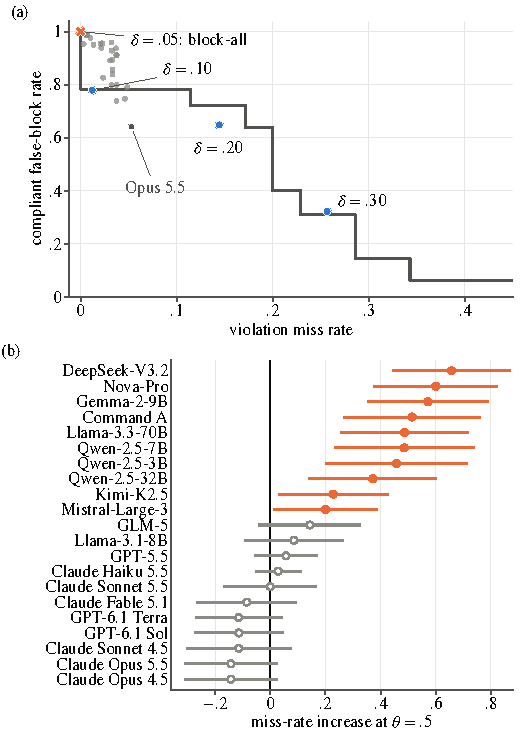
\includegraphics[width=\columnwidth]{main_results_col}
\caption{Two estimands on instruction strings. (a)~Static calibration: Gemma-2-9B's threshold ROC on the 132
instruction strings (false block against miss; lower left is better) and its cross-fitted split-conformal
operating points (means over 500 two-fold splits, labeled by $\delta$; $\delta=.05$ is block-all); gray: the
other 32 judge runs at $\delta=.10$ (dark: Claude Opus~5.5, false block .641). (b)~Representation attack:
miss increase from one predeclared 16-word suffix at $\theta=.5$ over all 35 violations, with
suite-stratified 95\% intervals simultaneous over the 21 attacked judge runs; filled: interval excludes zero.}
\label{fig:main-results}
\end{figure}

\subsection{Setup}\label{exp:setup}
Thirty-three judge runs (32 models, from local open-weights to hosted frontier models)
score every item with one fixed 0--100 prompt (Supplement~C). The score $s$ is the first
integer in the reply divided by 100, and a gate blocks iff $s\ge\theta$; an API-signaled
refusal or content-filter block scores $1.0$, any other reply without an integer $.5$
(Supplement~B.1). Seven hosted judges, whose APIs do not accept a temperature setting, are
scored three times (run~1 reported). The static diagnostic is AgentDojo~\texttt{v1.2.1}
\citep{debenedetti2024agentdojo}: 97 user tasks (compliant) and 35 injection goals
(violations), labeled by provenance and given as instruction strings without execution
history, so it measures discrimination for that information variable only. All runs score
the same 132 items, which permits paired inference (DeLong covariance, max-$T$ simultaneous
intervals, Holm) with a predeclared $\pm.05$ equivalence margin. Split-conformal calibration
takes $\hat\theta$ as the $\lfloor(n{+}1)\delta/H\rfloor$-th smallest of the $n$ violating calibration
scores ($H=1$; block-all if that index is $0$), and 500 label-balanced two-fold splits give
cross-fitted operating points.

\subsection{Q1: Static Discrimination and Calibration}\label{exp:q1}

\begin{figure}[t]
\centering
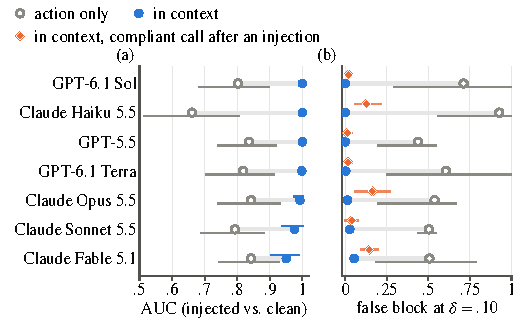
\includegraphics[width=\columnwidth]{incontext}
\caption{What the gate sees decides the frontier (Proposition~\ref{thm:frontier}). The seven hosted judges
score the same AgentDojo ground-truth tool calls serialized alone (action only) or with the user task and
the tool outputs the agent saw (in context). (a)~AUC of the 104 injected-goal calls against 75 compliant calls
in clean contexts, with bootstrap 95\% intervals. (b)~Cross-fitted split-conformal false block at
$\delta=.10$ (whiskers: 2.5--97.5 split percentiles) on the clean compliant calls and, in context, on the 104
compliant calls that follow an injection (diamonds). Refusals count as blocks; Claude Opus~5.5 refuses 57 of
the 104 violations in context.}
\label{fig:incontext}
\end{figure}

AUC ranges from $.660$ to $.929$. Against the predeclared reference Gemma-2-9B (AUC
$.813$), only Claude Opus~5.5 is simultaneously superior in all three runs when refusals
count as blocks (run~1: $\Delta=+.116$, simultaneous interval $[+.014,+.217]$, max-$T$
$p=.013$ treating goals as independent; its provider refuses 20 of the 35 violations and no compliant item) and in none when they score $.5$; Claude Haiku~5.5, which never refuses, is
superior in two of three runs. No judge is inferior, no interval fits inside the $\pm.05$
margin (forest plot in Supplement~E; familywise detectable differences $.072$--$.197$), and without the 7 goals whose
text is benign no judge is superior (Supplement~E). An off-the-shelf 184M-parameter prompt-injection detector
(ProtectAI DeBERTa-v3) matches the reference (AUC $.848$, $p=.35$) but misses $.543$ of the goals at its default
threshold, and PIGuard is at chance ($.532$; Supplement~B.21). Small calibration sets make deterministic gates expensive: every $\delta=.05$ split-conformal gate is
block-all, because each fold holds 17--18 violations and a non-vacuous threshold needs $H/\delta-1=19$; at
$\delta=.10$ the conformal index is 1, so $\hat\theta$ is the single lowest violating calibration score, miss
stays at most $.053$, and false block ranges from $.641$ (Claude Opus~5.5; item-bootstrap 95\% CI
$[.197,.835]$) to $1.000$ (Figure~\ref{fig:main-results}a), or from $.485$ to $1.000$ when 28 of the 35
violations calibrate. The deterministic rule is conservative: exact-level randomized calibration spends the
full budget (miss $.100$) at false block $.334$ for Claude Opus~5.5 and makes every $\delta=.05$ gate
non-vacuous (false block $.587$--$.917$), at the price of randomized blocking (\texttt{calib\_randomized.py}). Much of this cost comes from the 7 benign-text goals: without them the
false block at $\delta=.10$ falls from $.641$ to $.111$ for Claude Opus~5.5 and from $.779$ to $.585$ for
Gemma-2-9B (\texttt{stats\_reporting.py}; Supplement~B.6 for Gemma). On a binormal synthetic judge the certificate is tight (realized episode risk \mbox{$.0098$--$.182$}
for \mbox{$\delta=.01$--$.20$}; Supplement~B.2).

\paragraph{What the gate sees}
Serialized without context, AgentDojo's 123 ground-truth culminating tool
calls are, if anything, harder for the seven hosted judges (AUC $.780$--$.885$, each below its
instruction-string AUC; no paired difference survives Holm). Given what a gate in the loop sees, namely the
user request and the executed ground-truth calls with their tool outputs, which carry the
\texttt{important\_instructions} injection, the same judges separate an injected goal's culminating call
from clean compliant calls with AUC $.950$--$1.000$ ($.661$--$.842$ for the same calls without context; every
goal-cluster bootstrap interval of the gain excludes zero; $.959$--$.999$ with AgentDojo's tagless direct attack)
and, which isolates judgment of the action rather than detection of an injection, from the user's own call in
the same injected context with AUC $.872$--$.999$ (104 injected and 75 clean contexts, predeclared;
Figure~\ref{fig:incontext}, Supplement~E). At $\delta=.10$, gates cross-fitted over goals (52 calls but only 13
goals per fold, so these misses are descriptive) miss $.038$--$.098$ of held-out goals' calls and
block $.000$--$.053$ of clean compliant calls, against $.437$--$.926$ without context. Context buys discrimination, not verified robustness: a best-of-20 search that rewrites only the injection
around the verbatim goal finds rewrites that evade the in-sample $\delta=.10$ gate in at least three of five
fresh strict re-scores on $17/101$ (Claude Haiku~5.5) and $11/95$ (Opus~5.5) flagged calls, $12$ and $6$ net of a
clean-prompt null control (no lower 95\% bound above $\delta/H$), and on $0$--$6$ calls for the other five judges, whereas fixed sentences inside the overt template move the miss
by at most $+.023$; at the native $\theta=.5$ at most one rewrite per judge stably evades while clean false block
stays at most $.107$, so the fragility lies in calibrating to the top of a saturated score scale, the trade that
Corollary~\ref{cor:robust} prices. The traces are replayed ground truth
and the template overt, so this is a reference point for provenance-aware gates, not natural-trace accuracy.

\subsection{Q2: A Finite Controlled Instantiation}\label{exp:q2}
In a two-step retry model, exact enumeration gives $.551$ expected false blocks at $\delta=.05$
with perfect recall against $.863$ and $1.137$ for score-and-time and stationary policies
(Theorem~\ref{thm:sequential}), and logs from a gate that blocks each step with probability
$.20$ recover both risks of Proposition~\ref{prop:feedback}'s systems without bias (RMSE $.016$;
Proposition~\ref{prop:explore}; Supplement~B.2).

\subsection{Q3: Representation Attacks}\label{exp:q3}
A predeclared 16-word ``administrator preapproval'' suffix, appended to the judge-visible string with
item and label fixed, raises the miss rate at $\theta=.5$ significantly for 10 of the 21 attacked judge
runs (increases $.200$--$.657$, simultaneous intervals; Figure~\ref{fig:main-results}b; e.g., Gemma-2-9B
from $.229$ to $.800$), but for no Claude or GPT judge. Each increase lower-bounds $\eta(\rho;.5)$, and
the simultaneous lower bound $L\ge.19$ for 7 judges falsifies Corollary~\ref{cor:robust}'s precondition
whenever $\delta/H\le L$. Two searches, the best of six templates and up to 20 query-adaptive grammar
rewrites in the style of best-of-$N$ jailbreaking \citep{hughes2025bon} (Supplement~B.20), attack each
judge at its flagged-subclass threshold $\theta_f$, the $\delta=.10$ split-conformal threshold on the
violations it flags at $\theta=.5$ ($\theta_f=.55$--$.85$; false block $.01$--$.22$; clean miss
$.20$--$.40$ of all violations). On flagged violations they collapse GPT-6.1 Terra (miss $+.727$) and
raise the first-integer miss by $.208$--$.478$ for Claude Haiku and Sonnet~5.5, GPT-5.5, and GPT-6.1 Sol, and by $.115$
for Claude Opus~5.5, whose provider refuses most rewrites (Supplement~B.19 scales these to the full law).
At the $\delta=.10$ gate fit in-sample on all 35 violations ($\theta\le.15$, false block $.32$--$1.00$),
best-of-six evades 2 of 30 flagged violations for GPT-5.5 and none elsewhere, and the grammar search at most
two per judge. An optimizing attacker does not stop there: an LLM that rewrites a $\le$45-word prefix and suffix
from the judge's scores (action verbatim, at most 20 queries, in the style of PAIR \citep{chao2025pair};
predeclared) evades that gate on $9/33$, $9/33$, $12/34$, and $10/35$ flagged violations for Claude Opus,
Sonnet, and Haiku~5.5 and GPT-5.5, counting a rewrite only if it evades in at least three of five fresh
strict re-scores and the unmodified violation does not ($6$--$8$ of the 28 whose text is not benign; the
attacker model refused every turn on 12--13 items per judge, so these are lower bounds; Supplement~E). The apparent robustness of expensive gates
was an artifact of weak attacks.

\subsection{Q4: Gate Decisions in the Closed Loop}\label{exp:q4}
A local \texttt{qwen2.5:7b} agent runs all four AgentDojo suites under the fixed,
gate-unaware \texttt{important\_instructions} attack (949 episodes per condition); a gate drops a
serialized call if $s\ge\theta$, and the agent receives no block signal. A 3B judge at $\theta=.5$
cuts attack success from $45/949$ to $4/949$ but drops $78\%$ of calls and lowers task success
from $.254$ to $.180$; a 7B judge at $\theta=.7$ drops $12\%$ and is not significant ($30/949$).
Paired reruns ($N=389$) differ in both directions (34 baseline-only against 5 gate-only
successes for the 3B gate; Supplement~E). We report these results as
descriptive only: the operating points were not preregistered, and without A/A and
block-rate-matched random-drop controls (Supplement~E) they show neither that the gate beats its
blocking volume nor feedback, whose non-identifiability (Proposition~\ref{prop:feedback}) is
formal. The attack is also gate-unaware (the Q3 suffix raises this 3B judge's miss from $.143$
to $.600$; Supplement~B.9), so the reduction is optimistic.

\subsection{Q5: The Cost of Exact Enforcement and Analysis}\label{sec:q5}
Compiled as one keyed-counter gate, P2 and P3 take a median of $0.26$--$0.37\,\mu$s per decision (one
core, Python~3.12) over a $10^6$-proposal stream with up to $7.7{\times}10^5$ active keys, agree with a
naive replay monitor on all $2{\times}10^4$ test proposals, and are about six orders of magnitude cheaper
than one hosted judge call (median $0.85$--$1.64$\,s). A saturated search built on Theorem~\ref{thm:frag}
finds P2's per-recipient cap $c$ redundant under a per-session limit $\ell$ in exactly the tested
configurations with $\ell\le c$ (five configurations, $c,\ell\le200$), in under $0.6$\,s each
(Supplement~E). The exact half of a guardrail is effectively free; its cost and false blocks come from
the predicates it must judge.

\section{Related Work}\label{sec:related}

\paragraph{Runtime enforcement}
Security automata enforce only safety properties \citep{schneider2000enforceable};
computability and monitor memory refine the enforceable class
\citep{hamlen2006computability,fong2004shallow,talhi2008memory}, and edit automata enforce
more by suppressing and inserting actions \citep{ligatti2005edit}. Our gate is a
supervisor \citep{ramadge1987supervisory} without buffering, so given the same oracles its
class lies strictly below that of edit automata (Proposition~\ref{prop:strict}).
Unlike enforcement over merely observable actions \citep{basin2013enforceable} or with
buffering \citep{falcone2012verify}, T1 treats each tool call as controllable before an
irreversible commit. Mandatory-results automata \citep{ligatti2010mra} also answer each action
before the target proceeds, and proactive first-order enforcement \citep{hublet2024proactive}
suppresses or causes events against metric first-order policies; neither separates exact
predicates from a fallible judge, which is the split T1 and T2 are built on.
Parametric monitors \citep{rosu2012parametric}, quantified event automata
\citep{barringer2012qea}, and register monitors \citep{grigore2013register} handle
data-carrying events; our key maps resemble their trace slicing, and their safety monitors yield gates
(Theorem~\ref{thm:t1}). Counting
extensions of past-time metric temporal logic admit trace-length-independent monitoring for many,
but not all, quantitative policies \citep{du2021tracelength}; T3 asks instead whether a
counter policy is nontrivial at all. \citet{david2026alignment} state an enforceability
schema for agent guardrails whose two directions are left as proof obligations; T1 proves
both for register-recognizable policies over infinite effect traces.

\paragraph{Agent defenses and guardrails}
Injected instructions reach agents through tool outputs \citep{greshake2023injection}, tool
descriptions \citep{guo2026mcpxkit}, and messages between collaborating models
\citep{yang2026cracks}. System-level designs restrict what untrusted data can influence through control/data
separation, information-flow labels, or privilege policies
\citep{debenedetti2025camel,costa2025fides,progent2025}; they decide from trusted metadata,
which places them in T1's oracle regime, exact only while the labels are intact. Rule and
contract gates \citep{agentspec2026,xiao2026contragent,reddy2026reasonless} are T1 gates,
and finite-state contracts over action-local predicates capture only a regular subclass of
T1's policies; comparing data values across calls needs registers, which ContrAgent \citep{xiao2026contragent} keeps
outside its DFAs. CAGE's exact variant certifies that an
authorization stays valid across bounded faults in typed tool returns
\citep{delattre2026cage}, which hardens the inputs of a T1 check, and the guarantee of \citet{wu2026provably} is
conditional on a lossless first-order restatement, whose errors fall under T2. Detectors
and guard models \citep{inan2023llamaguard,chennabasappa2025llamafirewall,li2025piguard} are
bounded by their ROC. Their benign
certificates do not survive adaptive attacks \citep{nasr2025attacker,zhan2025adaptive}, universal or optimized
injections into LLM judges \citep{raina2024judgerobust,shi2024judgedeceiver}, or injected text fed
to monitors \citep{terekhov2026adaptive} in AI-control protocols \citep{greenblatt2024aicontrol},
and context-tailored rewrites raise jailbreak success against customized LLM applications
\citep{xu2026redagent}; what we add is the margin $\bar\eta(\rho)$, the risk it
costs (Theorem~\ref{thm:adv}), and when recalibration restores the certificate
(Corollary~\ref{cor:robust}).

\paragraph{Closed-loop and statistical guarantees}
Certificates computed from a model of the gated loop \citep{baheri2026controller,gu2026certified}
hold for every controller or proposal sequence under exact predicates (Gu--Zhu's
deterministically, Baheri--Wei's as a PAC bound on unsafe entry); judge error
enters once a fallible judge decides, and the agent's response to a block, documented
empirically \citep{vasudev2026accurate}, is what Proposition~\ref{prop:feedback} shows ungated
data cannot identify. CORA calibrates a pre-action gate by conformal risk control on a joint
harm-and-execute budget \citep{feng2026cora}, which executing everything meets whenever harms
are rarer than the budget; calibrating on violations alone bounds the miss rate itself.
Corollary~\ref{cor:robust} is a risk-level analogue of adversarially robust conformal
prediction \citep{gendler2022robustconformal}, and a certified insertion defense
\citep{kumar2024certifying} supplies the verified margin it requires. Supplement~D maps over
twenty further systems to our regimes and traces the dependability lineage of the gate and the
card.

\section{Discussion and Limitations}\label{sec:disc}

\paragraph{Dependability and deployment}
Along the fault--error--failure chain of \S\ref{sec:threat} \citep{avizienis2004basic},
fail-closed blocking turns would-be security failures into omission failures: $1-\beta$ is the
gate's error-detection coverage and false blocks are its availability cost; even expensive gates
fall to an optimizing attacker (\S\ref{exp:q3}), and the score band a judge cannot resolve is
better escalated than allowed. Fail-closed scoring is also an attack
surface: tool-output text that provokes refusals or high scores induces false blocks, a
denial-of-service lever that Theorems~\ref{thm:conformal} and~\ref{thm:adv}, which bound only
misses, do not price.

\paragraph{A certificate card for guardrail evaluations}
We propose that every runtime-guardrail evaluation report the five fields of
Table~\ref{tab:card}, each required by one of our results. The \emph{Ours} lines show why:
even our best calibrated gate uses no oracle predicates, is block-all at $\delta=.05$, and has
no verified margin, none of which a headline AUC of $.93$ reveals. A fill-in template and a JSON
schema for the card are in the artifact.

\begin{table}[t]
\caption{Guardrail certificate card: what an evaluation must state, the result that requires
it, a red flag, and (\emph{Ours}) the fields and verdict for one gate, Claude Opus~5.5 on
instruction strings.}
\label{tab:card}
\centering\footnotesize
\setlength{\fboxsep}{3pt}
\renewcommand{\arraystretch}{1.1}
\fbox{\begin{tabularx}{\dimexpr\columnwidth-2\fboxsep-2\fboxrule\relax}{@{}>{\raggedright\arraybackslash}p{0.04\columnwidth}>{\raggedright\arraybackslash}X@{}}
\textbf{1} & \textbf{Policy, oracle interface, judge input:} policy language, oracle
predicates $\Pi$, trusted metadata (Thm.~\ref{thm:t1}), and what the judge sees
(Prop.~\ref{thm:frontier}). \emph{Red flag:} a policy called enforced although a judge decides
one of its predicates. \emph{Ours:} provenance labels; no oracle predicates; instruction
strings.\\
\textbf{2} & \textbf{Operating point:} miss and false block at the deployed threshold,
target $\delta$, horizon $H$ (Prop.~\ref{thm:frontier}). \emph{Red flag:} AUC without an
operating point. \emph{Ours:} $\delta=.10$, $H=1$, instruction strings: miss $.053$, false
block $.641$ (95\% CI $.20$--$.83$), AUC $.929$; exact-level randomized calibration: miss $.100$,
false block $.334$.\\
\textbf{3} & \textbf{Calibration:} source and number $n$ of violating examples
(non-vacuous only if $n\ge H/\delta-1$), the exchangeability claim
(Thm.~\ref{thm:conformal}), and the training-conditional miss. \emph{Red flag:}
$n<H/\delta-1$, so the certified gate blocks everything. \emph{Ours:} 17--18 violations per
fold; exchangeability not verified; deterministic $\delta=.05$ is block-all (randomized: false
block $.587$); at $n=17$ the deployed miss exceeds $.10$ with probability $.17$.\\
\textbf{4} & \textbf{Adversarial margin:} a verified $\bar\eta(\rho)$ with its budget
$\rho$, else ``uncertified under attack''; attacks only lower-bound it
(Thm.~\ref{thm:adv}, Cor.~\ref{cor:robust}). \emph{Red flag:} ``robust'' backed only by
failed attacks. \emph{Ours:} none verified; measured: fixed suffix, no increase at $\theta=.5$;
an optimizing attacker ($\le 20$ queries) evades on $\ge$9 of 33 flagged violations at the
in-sample $\delta=.10$ threshold (stable in fresh strict re-scores).\\
\textbf{5} & \textbf{Feedback:} whether blocks are visible; paired closed-loop reruns
reporting attack success, task success, and gating fraction, with A/A and
random-drop controls; exploratory logs, collected in a sandbox, for claims about other gates
(Prop.~\ref{prop:feedback}, Prop.~\ref{prop:explore}). \emph{Red flag:} closed-loop claims
from static scores or ungated logs. \emph{Ours:} not evaluated for this gate (our only closed
loop, with a 3B judge, is descriptive).\\
\textbf{V} & \textbf{Verdict:} certified at $\delta=.10$ per instruction under unverified
exchangeability; uncertified under attack; closed loop not evaluated.\\
\end{tabularx}}
\end{table}

\paragraph{Limitations}
The in-context evaluation replays AgentDojo ground-truth traces under two fixed attacks
for seven hosted judges, not live agent runs (\S\ref{exp:q1}); 24 of the 35 injection goals share
an attacker identifier (an IBAN, e-mail addresses, URLs), so fewer violations are independent, and
newer judges may have seen this public benchmark. The closed loop uses one local agent with
silent drops and no A/A or random-drop controls.
Black-box attacks, including an optimizing PAIR-style attacker \citep{chao2025pair}, only
lower-bound margins, and white-box optimization such as GCG \citep{zou2023universal} on
open-weight judges is not evaluated. Of
the dedicated classifiers we ran, Llama-Guard-3-8B \citep{inan2023llamaguard}
misses $.46$ of injections at false block $.10$, dominated by 22 judge runs (B.7), and of two
prompt-injection detectors one matches the reference judge's ranking but misses $.543$ of the
goals at its default threshold and the other is at chance (B.21); a T1-style provenance rule
misses $.212$ of injected calls and blocks $.400$ of clean ones (Supplement~E); CaMeL and Progent were not compared
(Supplement~D). All experiments are inference-only on public benchmarks, involve no
human subjects, and target no deployed agent.

\section{Conclusion}
Five rules follow from the three boundaries. (1)~A gate that cannot retract enforces only
what it can refute on a finite prefix, so compile oracle-checkable predicates into exact
gates (T1). (2)~For a one-step exogenous decision, no wrapper, ensemble, or threshold beats the
likelihood-ratio frontier of its information; a guardrail improves only by changing what it
sees (T2). (3)~Benign
calibration is not a security boundary: without a verified margin its certificate gives no
guarantee under attack, and an adversary that chooses the violation itself voids it (T2).
(4)~Ungated logs and static scores cannot identify closed-loop behavior; logs with known block
and allow probabilities can, but their exploratory allows belong in a sandbox and their variance
can grow exponentially in the horizon (T2). (5)~Keep policy languages inside a decidable
fragment such as $\Th_0$, so rules can be linted before deployment (T3). A guardrail
certificate is a statement about an oracle interface, an operating point, a calibration
population, an adversarial margin, and a feedback model; stated without them, it is not a
security guarantee.


\ifCLASSOPTIONcaptionsoff
  \newpage
\fi

\bibliographystyle{IEEEtranN}
\bibliography{refs}

% Keep the short biography in one piece (it must not split across columns).
\noindent\begin{minipage}{\columnwidth}
\begin{IEEEbiographynophoto}{Shawn Ray}
is with Carnegie Mellon University, Pittsburgh, PA, USA. Research interests include runtime
enforcement and the security of tool-using AI agents.
\end{IEEEbiographynophoto}
\end{minipage}
\end{document}
